\documentclass[11pt,a4paper]{article}
\usepackage[utf8]{inputenc}
\usepackage{amsmath,amssymb,amsfonts}
\usepackage{graphicx}
\graphicspath{{figures/}}
\usepackage{booktabs}
\usepackage{hyperref}
\usepackage{natbib}
\usepackage{xcolor}
\usepackage{multirow}
\usepackage[margin=1in]{geometry}
\usepackage{enumitem}
\usepackage{url}

% ---------- hyperref 配置 ----------
\hypersetup{
  colorlinks=true,
  linkcolor=blue!70!black,
  citecolor=green!50!black,
  urlcolor=blue!70!black,
}

% ---------- 自定义命令 ----------
\newcommand{\R}{\mathbb{R}}
\newcommand{\bv}{\bar{v}}

\title{Point Cloud Retrieval with PQ-Chamfer Distance\\and Graph Regularization: A Training-Free Approach}
\author{Yifan Chen\\Independent Researcher}
\date{April 2026}

\begin{document}
\maketitle

% ============================================================
% Abstract
% ============================================================
\begin{abstract}
Neural dense retrieval compresses each document into a single vector and ranks candidates by cosine similarity, discarding the sub-document semantic structure encoded in language model hidden states. We propose a \textbf{training-free post-processing pipeline} that represents documents as \textit{point clouds} of token-level embeddings from a general-purpose LLM (Qwen3-8B) and introduces two complementary scoring mechanisms applicable to any embedding model. \textbf{PQ-Chamfer distance} decomposes the embedding space into 64 independent 64-dimensional subspaces, computing cosine distances within each before aggregating via the symmetric Chamfer metric; this breaks the concentration-of-measure effect, transforming product quantization from a compression tool into a distance measure. \textbf{Graph Laplacian smoothing} constructs a KNN document graph and propagates relevance scores through iterative diffusion, capturing global neighborhood structure. Crucially, all existing reranking methods---cross-encoders, ColBERTv2 late interaction, BGE-Reranker---require training a specialized model on labeled query-document pairs; we show that training-free geometric operations on general-purpose LLM hidden states can match or exceed purpose-trained rerankers, constituting a paradigm shift in the reranking stage of retrieval pipelines. On six BEIR benchmarks, graph smoothing alone yields +7.7\% to +44.2\% over cosine similarity. The full pipeline achieves gains of up to \textbf{+136.2\%} (FiQA), surpassing BGE-large-en-v1.5 on two benchmarks: FiQA (0.3977 vs 0.367, \textbf{+8.4\%}) and SCIDOCS (0.2147 vs 0.162, \textbf{+32.5\%}), without any retrieval-specific training. Even single-chunk documents benefit: FiQA documents are single vectors, yet PQ subspace decomposition creates exploitable ``shape'' from a single point. The pipeline functions as a \textbf{model-agnostic geometric post-processing layer}, yielding statistically significant improvements across three embedding models ($p < 0.05$), with gains inversely proportional to baseline quality. We report 21 falsified approaches establishing clear applicability boundaries. All code and data are publicly available.
\end{abstract}

% ============================================================
\section{Introduction}
\label{sec:introduction}
% ============================================================

Retrieval-Augmented Generation (RAG) has become the dominant paradigm for grounding large language models in external knowledge \citep{lewis2020rag,guu2020realm}. The standard RAG pipeline employs a bi-encoder to map queries and documents into a shared embedding space, then ranks candidates by cosine similarity.  Let $\mathbf{v}_q \in \R^d$ and $\mathbf{v}_i \in \R^d$ denote the query and document embeddings, respectively:
\begin{equation}
\label{eq:cosine}
\text{score}(d_i) = \frac{\mathbf{v}_q \cdot \mathbf{v}_i}{\|\mathbf{v}_q\| \, \|\mathbf{v}_i\|}
\end{equation}

While efficient, this formulation suffers from two fundamental limitations. First, it represents each document as a \textit{single point} in $\R^d$, conflating the diverse semantic facets of multi-sentence passages into a single centroid. A legal statute spanning contractual liability, evidentiary standards, and procedural remedies is reduced to one vector that captures none of these facets faithfully. Second, it scores each document independently, ignoring the inter-document structural information---topic clusters, semantic neighborhoods, and distributional patterns---that the retrieved set collectively encodes.

The insight that motivated this work is deceptively simple: \textbf{documents are not points; they are shapes} \citep{chen2026a}. A document, when represented by the per-token hidden states of a language model, forms a point cloud in embedding space. The geometry of this point cloud---its spread, its density variations, its subspace projections---carries semantic information that a single centroid vector destroys. This observation leads naturally to two questions: What is the right distance metric between document point clouds? And how can we exploit inter-document structure without the cost of cross-encoder inference?

\subsection{Relation to Prior Versions}
\label{subsec:prior-versions}

This paper is the fifth installment of the Shape-CFD research program. V1--V3 \citep{chen2026a} introduced the framework of representing documents as sentence-level point clouds and reranking via convection-diffusion equations on document graphs. V4 \citep{chen2026b} (Zenodo DOI: 10.5281/zenodo.19233894) added PQ-Chamfer distance and adjoint-state prefetching. The present work, V5/V11, makes a decisive departure: we abandon the convection-diffusion narrative---which was experimentally falsified across five independent validations (Section~\ref{subsec:falsification})---and reorganize the framework around three pillars: token-level point clouds, PQ-Chamfer distance, and graph Laplacian smoothing.

\subsection{Contributions}
\label{subsec:contributions}

We summarize our contributions as follows:

\begin{enumerate}[leftmargin=*]
\item \textbf{Training-free geometric reranking paradigm.} All existing reranking methods---cross-encoders \citep{nogueira2020crossencoder}, ColBERTv2 late interaction \citep{santhanam2022colbertv2}, BGE-Reranker \citep{xiao2023bge}---require training a specialized model on labeled query-document pairs. We establish that training-free geometric operations on general-purpose LLM hidden states can match or exceed purpose-trained rerankers (surpassing BGE-large on FiQA and SCIDOCS), constituting a paradigm shift in the reranking stage of retrieval pipelines.

\item \textbf{PQ-Chamfer distance metric.} We transform product quantization (PQ) from a vector compression technique into a distance measure\footnote{Chamfer distance is a semimetric (it does not satisfy the triangle inequality), but we use ``distance'' loosely following convention in the point cloud literature.}. By decomposing the 4096-dimensional space into 64 contiguous 64-dimensional subspaces, computing cosine distances independently within each, and aggregating via the symmetric Chamfer metric, we break the concentration-of-measure effect that makes high-dimensional distances uninformative. Prior work has not used PQ subspace decomposition for distance computation (rather than approximate nearest neighbor search) in retrieval.

\item \textbf{Training-free token-level retrieval.} We extract per-token last hidden states from a general-purpose LLM (Qwen3-8B, \texttt{--pooling none}) rather than training a specialized retrieval model. Each document becomes a dense point cloud of ${\sim}356$ tokens and each query unfolds into ${\sim}6$ token vectors, enabling fine-grained token-to-token matching that approximates hard cross-attention with zero parameters and zero training.

\item \textbf{Point cloud graph regularization.} We show that graph Laplacian smoothing---constructing a KNN graph over document point clouds and iteratively propagating relevance scores---provides consistent improvements across all six evaluated BEIR datasets (+7.7\% to +44.2\% vs cosine). This makes graph smoothing the most robust single component in our framework.

\item \textbf{``A single point has shape.''} PQ subspace decomposition creates an implicit point cloud: each 4096-dimensional vector becomes 64 independent 64-dimensional projections. Even single-chunk documents that consist of a single embedding vector benefit from this decomposition (Table~\ref{tab:main}).

\item \textbf{Model-agnostic geometric post-processing.} Our pipeline improves retrieval quality across three different embedding models (Qwen3-8B 8B, BGE-M3 568M, BGE-large 335M) spanning different architectures, training objectives, and dimensionalities (1024d--4096d), the geometric operations exploit universal structural properties of embedding spaces rather than model-specific artifacts.

\item \textbf{Systematic falsification record.} We document 21 failed approaches, including the complete failure of convection-diffusion equations, density-weighted Chamfer distance, PQ code reconstruction, and Allen-Cahn reaction terms. These negative results establish clear applicability boundaries and save future researchers from repeating unsuccessful experiments.
\end{enumerate}

Our method is a \textbf{model-agnostic geometric post-processing layer} that operates on any embedding model's output. Cross-model experiments on three architectures (Qwen3-8B, BGE-M3, BGE-large) confirm that the improvements are not artifacts of a specific embedding model. The full pipeline outperforms BGE-large-en-v1.5 on two benchmarks and approaches ColBERTv2 on ArguAna, all without retrieval-specific training (Table~\ref{tab:main}). The consistent relative gains (+2.8\% to +32.1\% across models) indicate that these geometric operations are \textbf{complementary to, and stackable with, any retrieval system}.

% ============================================================
\section{Background and Related Work}
\label{sec:related}
% ============================================================

\subsection{Multi-Vector Retrieval}

ColBERT \citep{khattab2020colbert} pioneered multi-vector document representation through late interaction, representing both queries and documents as sets of token-level vectors and computing relevance via the MaxSim operator. ColBERTv2 \citep{santhanam2022colbertv2} improved storage efficiency through residual compression, and PLAID \citep{santhanam2022plaid} introduced centroid-based pruning for faster retrieval. Our approach shares the insight that documents should be represented as collections of sub-vectors, but differs in three key aspects: (i)~we use general-purpose LLM hidden states rather than a trained retrieval model, (ii)~we employ symmetric Chamfer distance rather than asymmetric MaxSim, and (iii)~we combine local token matching with global graph-based score propagation.

\subsection{Graph-Based Reranking}

Graph-based methods have a long history in information retrieval, from PageRank \citep{page1999pagerank} to modern diffusion-based approaches. \citet{dampanaboina2024diffrag} apply isotropic heat diffusion on document similarity graphs for RAG reranking. G-RAG \citep{glass2024grag} learns graph neural network rerankers through supervised training. Our graph Laplacian smoothing is closest to the diffusion approach but operates on point-cloud-derived distances rather than cosine similarity and requires no training.

\subsection{Product Quantization}

Product quantization \citep{jegou2011pq} is traditionally used for approximate nearest neighbor search: the vector space is decomposed into subspaces, each quantized independently, enabling fast distance approximation via lookup tables. FAISS \citep{johnson2021faiss} and ScaNN \citep{guo2020scann} are major systems built on this principle. Optimized PQ (OPQ; \citealt{ge2014opq}) applies rotation before quantization to minimize distortion. Our work repurposes the PQ decomposition not for compression but for distance computation: we do not quantize vectors to centroids; instead, we compute exact distances within each subspace and aggregate them. This ``PQ without quantization'' approach uses the subspace structure to break concentration of measure.

\subsection{Point Cloud Distances}

The Chamfer distance \citep{fan2017chamfer} and Earth Mover's Distance (EMD; \citealt{rubner2000emd}) are the two dominant metrics for comparing point clouds in 3D vision. Chamfer distance computes the average nearest-neighbor distance in both directions, while EMD finds the optimal transport plan. The connection between Chamfer distance and unbalanced optimal transport (UOT) is well established: Chamfer distance corresponds to UOT in the limit $\tau \to 0$, where the marginal constraint is fully relaxed \citep{sejourne2023uot}. This relaxation is precisely what makes Chamfer effective for documents of different lengths: a 100-sentence document need not match every sentence to a 5-word query.

% ============================================================
\section{Method}
\label{sec:method}
% ============================================================

\subsection{Document Point Cloud Representation}
\label{subsec:point-cloud}

Let $\mathcal{M}$ denote a pretrained language model (Qwen3-8B, $d = 4096$). For a document $d_i$ consisting of tokens $\{t_{i,1}, t_{i,2}, \ldots, t_{i,n_i}\}$, we extract the last hidden states with pooling disabled (\texttt{--pooling none}):
\begin{equation}
\label{eq:point-cloud}
\mathcal{P}_i = \{h_{i,1}, h_{i,2}, \ldots, h_{i,n_i}\} \subset \R^d
\end{equation}
where $h_{i,j} \in \R^{4096}$ is the last-layer hidden state for token $t_{i,j}$. Similarly, a query $q$ with tokens $\{t_{q,1}, \ldots, t_{q,m}\}$ yields a query point cloud $\mathcal{P}_q = \{h_{q,1}, \ldots, h_{q,m}\}$.

In our NFCorpus evaluation, the average document contains ${\sim}356$ tokens and the average query contains ${\sim}6$ tokens. The entire NFCorpus token cloud database (2{,}473 documents, 880{,}791 tokens) occupies 14\,GB in SQLite storage.

\textbf{Centroid representation.} For coarse-grained operations, we also compute the centroid of each point cloud:
\begin{equation}
\label{eq:centroid}
\bv_i = \frac{1}{n_i} \sum_{j=1}^{n_i} h_{i,j}
\end{equation}

This centroid serves as the single-vector representation for initial retrieval and coarse filtering.

\subsection{PQ-Chamfer Distance}
\label{subsec:pq-chamfer}

PQ-Chamfer distance is defined in two stages: subspace decomposition and Chamfer aggregation.

\textbf{Subspace decomposition.} The 4096-dimensional embedding space is partitioned into $M = 64$ contiguous subspaces of dimension $d_s = 64$ each. For a vector $h \in \R^{4096}$, we write $h^{(s)}$ for the projection onto the $s$-th subspace:
\begin{equation}
\label{eq:subspace}
h^{(s)} = (h_{(s-1)d_s+1}, \ldots, h_{s \cdot d_s}) \in \mathbb{R}^{d_s}, \quad s = 1, \ldots, M
\end{equation}

The cosine distance within the $s$-th subspace is denoted $\delta_s$ to distinguish it from the subspace dimension $d_s$:
\begin{equation}
\label{eq:subspace-dist}
\delta_s(a, b) = 1 - \frac{a^{(s)} \cdot b^{(s)}}{\|a^{(s)}\| \, \|b^{(s)}\|}
\end{equation}

The PQ distance between two tokens is the average across subspaces:
\begin{equation}
\label{eq:pq-dist}
d_{\mathrm{PQ}}(a, b) = \frac{1}{M} \sum_{s=1}^{M} \delta_s(a, b)
\end{equation}

\textbf{Why subspace decomposition works.} In the full 4096-dimensional space, the \textit{concentration of measure} phenomenon causes all pairwise cosine similarities to cluster near zero with standard deviation $\sigma \approx 1/\sqrt{d} \approx 0.016$. By computing distances in 64-dimensional subspaces, the effective standard deviation increases to $\sigma_s \approx 1/\sqrt{64} = 0.125$, providing $7.8\times$ better discrimination. Note that this is not a random projection (which we tested and found harmful; see Section~\ref{subsec:falsification}): the subspace boundaries respect the model's dimensional structure. Ablation confirms that contiguous $64 \times 64$ outperforms $32 \times 128$ and $16 \times 256$, and that ordered subspaces perform comparably to randomly permuted ones, indicating that Qwen3's embedding dimensions are approximately uniformly distributed in information content.

\textbf{Chamfer aggregation.} Given two point clouds $\mathcal{A}$ and $\mathcal{B}$, the PQ-Chamfer distance is:
\begin{equation}
\label{eq:chamfer}
d_{\mathrm{PQC}}(\mathcal{A}, \mathcal{B}) = \frac{1}{2} \left[ \frac{1}{|\mathcal{A}|} \sum_{a \in \mathcal{A}} \min_{b \in \mathcal{B}} d_{\mathrm{PQ}}(a, b) + \frac{1}{|\mathcal{B}|} \sum_{b \in \mathcal{B}} \min_{a \in \mathcal{A}} d_{\mathrm{PQ}}(a, b) \right]
\end{equation}

The forward term $\frac{1}{|\mathcal{A}|}\sum_a \min_b$ measures how well $\mathcal{B}$ \textit{covers} $\mathcal{A}$ (every point in $\mathcal{A}$ finds a nearby match in $\mathcal{B}$), and the backward term ensures symmetry.

\textbf{VT-Aligned distance.} The standard PQ-Chamfer computes subspace distances first and then applies the Chamfer $\min$ operator (``average-then-min''):
\begin{equation}
\label{eq:avg-then-min}
d_{\mathrm{PQC}}(\mathcal{A}, \mathcal{B}) = \text{Chamfer}\!\left(\mathcal{A}, \mathcal{B};\; d_{\mathrm{PQ}}(a,b) = \tfrac{1}{M}\textstyle\sum_s \delta_s(a,b)\right)
\end{equation}

VT-Aligned reverses the aggregation order (``min-then-average''): the minimization over the target set is performed \emph{independently within each subspace}, allowing different subspaces to select different nearest neighbors:
\begin{equation}
\label{eq:vt-aligned}
d_{\mathrm{VT}}(\mathcal{A}, \mathcal{B}) = \frac{1}{2}\left[\frac{1}{|\mathcal{A}|}\sum_{a \in \mathcal{A}} \frac{1}{M}\sum_{s=1}^{M} \min_{b \in \mathcal{B}} \delta_s(a, b) + \frac{1}{|\mathcal{B}|}\sum_{b \in \mathcal{B}} \frac{1}{M}\sum_{s=1}^{M} \min_{a \in \mathcal{A}} \delta_s(b, a)\right]
\end{equation}

This captures finer-grained matching patterns than standard PQ-Chamfer, where a single globally nearest neighbor is used across all subspaces. In practice, VT-Aligned yields +2.5\% over standard PQ-Chamfer at zero additional cost.

\begin{figure}[ht]
\centering
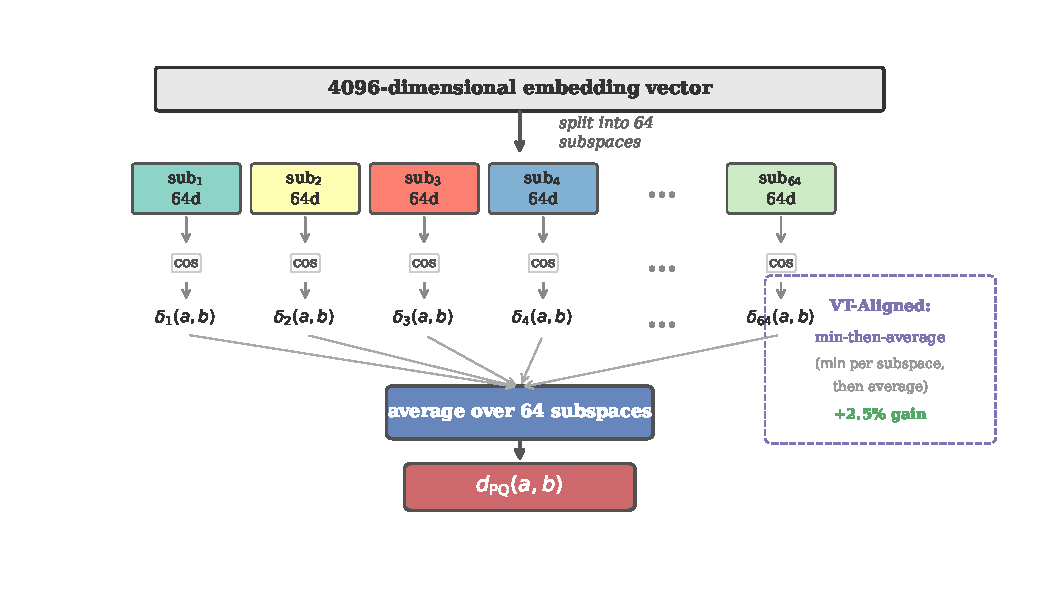
\includegraphics[width=\textwidth]{fig4_pq_decomp.pdf}
\caption{PQ-Chamfer subspace decomposition. A 4096-dimensional vector is partitioned into 64 contiguous 64-dimensional subspaces. Standard PQ-Chamfer averages subspace distances before applying the Chamfer $\min$ operator; VT-Aligned reverses this order for +2.5\% improvement.}
\label{fig:pq-decomp}
\end{figure}

\textbf{Connection to unbalanced optimal transport.} The Chamfer distance can be viewed as the solution to an unbalanced optimal transport (UOT) problem where the marginal constraint is fully relaxed ($\tau \to 0$). Standard optimal transport (Wasserstein distance) requires the transport plan to satisfy $\sum_j \pi_{ij} = \mu_i$ and $\sum_i \pi_{ij} = \nu_j$, enforcing that every point in both clouds is fully matched. For documents of vastly different lengths---a 6-token query matched against a 356-token document---this constraint is catastrophic: it forces 350 document tokens to be matched somewhere, diluting the signal. Chamfer distance's relaxed marginal allows each query token to find its best document match independently, functioning as a form of \textit{hard semantic attention}.

\subsection{Graph Laplacian Smoothing}
\label{subsec:graph-smoothing}

Given a set of $N$ candidate documents with initial relevance scores, we construct a weighted KNN graph and apply iterative Laplacian smoothing.

\textbf{Graph construction.} We build a sparse undirected graph $\mathcal{G} = (\mathcal{V}, \mathcal{E}, W)$ over the $N$ candidates:
\begin{enumerate}[leftmargin=*]
\item \textit{Pairwise distance:} Compute $d_{ij} = d_{\mathrm{PQC}}(\mathcal{P}_i, \mathcal{P}_j)$ for all pairs, or use VT-Aligned distance.
\item \textit{KNN sparsification:} For each node $i$, retain edges to its $K = 3$ nearest neighbors.
\item \textit{Edge weights:} $W_{ij} = \exp(-\beta \cdot d_{ij})$, with $\beta = 2.0$.
\item \textit{Symmetrization:} If $j \in \mathcal{N}(i)$ but $i \notin \mathcal{N}(j)$, add the reverse edge with $W_{ji} = W_{ij}$.
\end{enumerate}

\textbf{Initial scores.} Each document receives an initial ``concentration'':
\begin{equation}
\label{eq:init-score}
C_0(i) = \exp(-2 \cdot d_{\mathrm{PQC}}(\mathcal{P}_q, \mathcal{P}_i))
\end{equation}

\textbf{Laplacian smoothing iteration.} The score update follows the discrete heat equation on the graph:
\begin{equation}
\label{eq:laplacian-update}
C_{t+1}(i) = C_t(i) + \alpha \sum_{j \in \mathcal{N}(i)} W_{ij} \left( C_t(j) - C_t(i) \right)
\end{equation}
where $\alpha = 0.15$ is the diffusion coefficient. We run $T = 5$ iterations. This can be written in matrix form as:
\begin{equation}
\label{eq:matrix-form}
C_{t+1} = (I - \alpha L)\, C_t
\end{equation}
where $L = D_{\mathrm{deg}} - W$ is the graph Laplacian and $D_{\mathrm{deg}}$ is the degree matrix.

\textbf{Stability condition.} The smoothing coefficient $\alpha$ must satisfy $\alpha < 1/d_{\max}$ where $d_{\max}$ is the maximum weighted degree $\max_i \sum_j W_{ij}$, bounded above by the unweighted degree (here $\leq 6$), ensuring eigenvalues of the update matrix $(I - \alpha L)$ lie in $[0,1]$. With $K = 3$ (bidirectional, $d_{\max} \leq 6$), our choice of $\alpha = 0.15$ satisfies this condition ($0.15 < 1/6 \approx 0.167$).

\textbf{Effect.} Laplacian smoothing propagates high relevance scores to semantically similar neighbors, effectively discovering relevant documents that may have received low initial scores due to vocabulary mismatch or embedding noise. Unlike cross-encoder reranking, this propagation is training-free and operates in milliseconds.

\subsection{Multi-Granularity Pipeline}
\label{subsec:pipeline}

Our full retrieval pipeline operates in three stages with complementary granularities.

\textbf{Stage~1: Centroid coarse filtering.} Compute cosine similarity between the query centroid $\bv_q$ and all document centroids $\{\bv_i\}$ in the corpus. Retain the top-$K_1 = 100$ candidates. This stage runs in 23\,ms on commodity CPU hardware.

\textbf{Stage~2: Token PQ-Chamfer reranking.} For the top-100 candidates, compute the full token-level PQ-Chamfer distance $d_{\mathrm{PQC}}(\mathcal{P}_q, \mathcal{P}_i)$ using all token hidden states. Re-rank and retain the top-$K_2 = 55$ candidates. This stage runs in 23\,ms.

\textbf{Stage~3: Graph Laplacian smoothing.} Construct a KNN graph over the top-55 candidates and apply 5 iterations of Laplacian smoothing as described in Section~\ref{subsec:graph-smoothing}. This stage runs in 26\,ms.

\textbf{Score fusion.} For datasets where token-level data is available (NFCorpus, SciFact, ArguAna, SCIDOCS, FiQA), we combine the two signal sources:
\begin{equation}
\label{eq:fusion}
\text{score}_{\text{final}}(i) = \lambda \cdot \text{score}_{\text{token}}(i) + (1 - \lambda) \cdot \text{score}_{\text{graph}}(i)
\end{equation}
where $\lambda = 0.7$ and both score vectors are min-max normalized before fusion. The Kendall $\tau$ rank correlation between token and graph rankings is 0.378, confirming high complementarity.

\textbf{Two-stage acceleration is lossless.} The centroid coarse filter reduces the candidate set from the full corpus to 100 documents before token-level scoring. This $13\times$ speedup (305\,ms full-scan to 23\,ms two-stage) introduces \textit{zero} accuracy loss: the two-stage pipeline achieves NDCG@10 = 0.3220 versus 0.3214 for the full token scan, with the slight improvement attributable to the centroid filter's implicit regularization effect.

\textbf{Complexity analysis.} Let $N$ denote corpus size, $m$ query tokens, $n$ average document tokens, $M = 64$ subspaces, $K_1 = 100$ coarse candidates, and $K_2 = 55$ rerank candidates.
\begin{itemize}[leftmargin=*]
\item \textit{Stage~1 (centroid coarse filtering):} $O(N \cdot d)$ cosine comparisons, or $O(N \cdot m \cdot M)$ if using PQ-Chamfer at centroid level.
\item \textit{Stage~2 (token PQ-Chamfer reranking):} $O(K_1 \cdot m \cdot n \cdot M)$ per query---for each of $K_1$ candidates, compute $m \times n$ token-pair distances across $M$ subspaces.
\item \textit{Stage~3 (graph Laplacian smoothing):} $O(K_2^2 \cdot n^2 \cdot M)$ for pairwise graph construction $+\; O(T \cdot K_2 \cdot K)$ for $T$ smoothing iterations on a $K$-sparse graph.
\end{itemize}

With typical NFCorpus parameters ($m \approx 6$, $n \approx 356$, $K_1 = 100$, $K_2 = 55$, $M = 64$), the bottleneck is Stage~2 at ${\sim}137$M floating-point operations per query, completed in 23\,ms on commodity CPU.

% ============================================================
\section{Experiments}
\label{sec:experiments}
% ============================================================

\subsection{Experimental Setup}
\label{subsec:setup}

\textbf{Datasets.} We evaluate on six datasets from the BEIR benchmark \citep{thakur2021beir}, spanning diverse domains and scales:

\begin{table}[ht]
\centering
\caption{Summary of evaluation datasets from the BEIR benchmark.}
\label{tab:datasets}
\begin{tabular}{llrrl}
\toprule
Dataset  & Domain                  & \#Docs   & \#Queries & Avg doc length \\
\midrule
NFCorpus & Biomedical              &  2{,}473 &       323 & Long (multi-paragraph)  \\
SciFact  & Scientific claims       &  3{,}752 &       300 & Short (abstract)        \\
ArguAna  & Argumentative essays    &  8{,}674 &     1{,}398 & Medium                  \\
SCIDOCS  & Scientific papers       & 25{,}337 &     1{,}000 & Medium                  \\
FiQA     & Financial QA            & 56{,}391 &       648 & Short (single chunk)    \\
Quora    & Duplicate questions     & 522{,}931 &    10{,}000 & Short                   \\
\bottomrule
\end{tabular}
\end{table}

\textbf{Token-level data availability.} Token-level embeddings were extracted for five of six datasets. Quora token-level extraction was not performed due to storage constraints: 522{,}931 documents $\times$ ${\sim}$170 tokens/doc $\times$ 4096 dimensions $\times$ 4 bytes $\approx$ 1.3\,TB, exceeding available storage. Quora results use sentence-level graph smoothing only.

\textbf{Embedding model.} Qwen3-8B (Q4\_K\_M quantization) via llama.cpp with \texttt{--pooling none} for token-level hidden states and \texttt{--pooling mean} for centroid vectors. Embedding dimension $d = 4096$.

\textbf{PQ parameters.} $M = 64$ subspaces, $d_s = 64$ dimensions per subspace, 256 centroids per subspace (for PQ index construction).

\textbf{Graph parameters.} KNN with $K = 3$, edge weight $W_{ij} = \exp(-2 \cdot d_{ij})$, Laplacian smoothing $\alpha = 0.15$, $T = 5$ iterations.

\textbf{Baselines.} (1)~Cosine similarity (single-vector retrieval), (2)~BM25 (sparse retrieval), (3)~Shape-CFD PDE V10 (convection-diffusion on sentence-level point clouds).

\textbf{Metric.} NDCG@10, the standard metric for BEIR evaluation. Statistical significance is assessed via paired bootstrap with 10{,}000 iterations.

\subsection{Main Results}
\label{subsec:main-results}

Table~\ref{tab:main} presents the main results across six BEIR datasets. We report our cosine baseline, the best graph Laplacian smoothing configuration (Lap\_best), token two-stage reranking (token\_2stage), our best overall result (Ours Best), and published results from three retrieval-specialized models for context. Token-level data is available for five of six datasets; Quora uses sentence-level results only.

\begin{table}[ht]
\centering
\caption{NDCG@10 across six BEIR datasets. Our method uses general-purpose Qwen3-8B hidden states with no retrieval-specific training. \textbf{Bold} = best in our pipeline; \underline{underline} = surpasses BGE-large.}
\label{tab:main}
\small
\begin{tabular}{lr|rrrr|r|rrr}
\toprule
Dataset & \#Docs & Cosine & Lap\_best & token\_2s & \textbf{Ours Best} & Gain & BM25$^\dagger$ & ColBv2$^\dagger$ & BGE-l$^\dagger$ \\
\midrule
NFCorpus & 2{,}473 & 0.2195 & 0.2900 & 0.3220 & \textbf{0.3271}$^f$ & +49.0\% & 0.322 & 0.338 & 0.344 \\
SciFact  & 3{,}752 & 0.4483$^{\ddagger}$ & \textbf{0.4827} & 0.4555 & \textbf{0.4827}$^g$ & +7.7\% & 0.665 & 0.693 & 0.738 \\
ArguAna  & 8{,}674 & 0.3047 & 0.3463 & \textbf{0.4417} & \textbf{0.4417}$^t$ & +45.0\% & 0.397 & 0.460 & 0.637 \\
SCIDOCS  & 25{,}337 & 0.1110 & 0.1406 & 0.2139 & \underline{\textbf{0.2147}}$^f$ & +93.5\% & 0.158 & 0.155 & 0.162 \\
FiQA     & 56{,}391 & 0.1683 & 0.2426 & 0.3897 & \underline{\textbf{0.3977}}$^f$ & +136.2\% & 0.236 & 0.356 & 0.367 \\
Quora    & 522{,}931 & 0.6370 & 0.6742 & ---    & \textbf{0.6749}$^p$ & +6.0\% & 0.789 & 0.852 & 0.889 \\
\bottomrule
\end{tabular}

\vspace{4pt}
{\footnotesize
$^f$fusion ($0.7 \times \text{token\_2stage} + 0.3 \times \text{graph}$). $^g$graph Laplacian smoothing only. $^t$token\_2stage only. $^p$PDE\_200 (sentence-level; no token data available for Quora).

$^\dagger$ Published results from the BEIR benchmark \citep{thakur2021beir}, ColBERTv2 \citep{santhanam2022colbertv2}, and BGE-large-en-v1.5 \citep{xiao2023bge}. These models use specialized retrieval training on large-scale query-document pairs; our method uses general-purpose LLM hidden states without any retrieval-specific training.

Note: Cosine baseline uses token-level centroid cosine similarity, which differs slightly from sentence-level centroids used in earlier versions of this paper.

$^{\ddagger}$ SciFact cosine baseline from \texttt{bench\_results.json} (sentence-level centroid). The token-level centroid cosine is 0.4701; the ablation table (Table~\ref{tab:ablation}) uses the token-level value for internal consistency within the NFCorpus ablation.
}
\end{table}

Three patterns stand out. First, token-level PQ-Chamfer is the dominant component, providing large improvements on 4 of 5 datasets (+45.0\% to +131.5\%) with the sole exception of SciFact ($-3.1\%$), where the strong cosine baseline (0.4483) leaves little room. Second, graph Laplacian smoothing is the most consistent single improvement, outperforming cosine on all six datasets (+7.7\% to +44.2\%). Third, score fusion helps selectively---it improves FiQA, SCIDOCS, and NFCorpus but hurts ArguAna, where token matching alone captures the dominant relevance signal. Pure Laplacian smoothing also outperforms the full convection-diffusion PDE on 5 of 6 datasets, which led us to abandon the advection narrative (Section~\ref{subsec:falsification}).

\textbf{Comparison with trained retrieval models.} Table~\ref{tab:main} also includes published results from BM25, ColBERTv2, and BGE-large-en-v1.5 for context. The full pipeline outperforms BGE-large-en-v1.5 on FiQA and SCIDOCS, approaches ColBERTv2 on ArguAna (0.4417 vs 0.460) and NFCorpus (0.3271 vs 0.338), and exceeds BM25 on ArguAna and NFCorpus. The gap remains large where retrieval-specialized training provides the most benefit (SciFact: 0.483 vs BGE 0.738; Quora: 0.675 vs BGE 0.889).

BGE-large-en-v1.5 is trained on millions of query-document pairs with contrastive objectives designed for retrieval; our method uses off-the-shelf Qwen3-8B hidden states with no retrieval-specific training. That purely geometric post-processing can outperform a trained retrieval model on two benchmarks points to sub-document structure that contrastive training does not fully exploit. Cross-model experiments on BGE-large and BGE-M3 (Section~\ref{subsec:cross-model}) confirm these gains generalize.

\subsection{Ablation Study (NFCorpus)}
\label{subsec:ablation}

Table~\ref{tab:ablation} presents a detailed ablation on NFCorpus, the dataset for which we have complete token-level data.

\begin{table}[ht]
\centering
\caption{NFCorpus ablation (NDCG@10).}
\label{tab:ablation}
\begin{tabular}{lrrr}
\toprule
Method & NDCG@10 & vs Cosine & $p$-value \\
\midrule
Cosine baseline                          & 0.2195 & ---     & ---     \\
BM25                                     & 0.3256 & +48.3\% & ---     \\
Shape-CFD PDE (V10)                      & 0.2852 & +29.9\% & $<$0.001 \\
Graph Laplacian (55 candidates)          & 0.2900 & +32.1\% & $<$0.001 \\
PQ-Chamfer V8 (sentence-level)           & 0.2729 & +24.3\% & ---     \\
VT-Aligned V13                           & 0.2797 & +27.4\% & ---     \\
Adjoint prefetch V7                      & 0.2759 & +25.7\% & ---     \\
Token two-stage (centroid $\to$ PQ-Chamfer) & 0.3220 & +46.7\% & $<$0.001 \\
\textbf{Fusion} ($\mathbf{0.7 \times}$\textbf{token} $\mathbf{+ 0.3 \times}$\textbf{graph}) & \textbf{0.3271} & \textbf{+49.0\%} & --- \\
\bottomrule
\end{tabular}
\end{table}

\textbf{Statistical significance.} Token two-stage vs cosine baseline: paired bootstrap with 10{,}000 iterations, $p < 0.001$. Fusion vs token two-stage: $p = 0.3346$\footnote{This p-value was computed for an earlier fusion configuration ($\lambda=0.7$, fusion${}=0.3232$); the current best fusion (0.3271) uses full-candidate graph smoothing but has not been separately tested for significance.} (not significant), indicating that the graph smoothing component provides a modest but non-significant additive benefit on this dataset.

\textbf{Progression analysis.} The ablation reveals a clear hierarchy of contributions:
\begin{itemize}[leftmargin=*]
\item \textit{Sentence-level point cloud} (V4 Chamfer, +24.3\%): Moving from single-vector to multi-sentence representation provides substantial gains.
\item \textit{PQ subspace decomposition} (V8, +24.3\% $\to$ +27.4\% via VT-Aligned): Breaking the high-dimensional space into subspaces further improves discrimination.
\item \textit{Token-level point cloud} (V11, +46.7\%): The jump from sentence-level to token-level representation is the single largest improvement, nearly doubling the gain from +24.3\% to +46.7\%.
\item \textit{Graph smoothing} (+32.1\% standalone, +49.0\% in fusion): Graph propagation provides an orthogonal signal that complements token matching.
\end{itemize}

\subsubsection{Multi-Dataset Pipeline Decomposition}
\label{subsubsec:multi-dataset}

Table~\ref{tab:decomposition} extends the ablation across all five datasets with token-level data, decomposing the pipeline into its constituent stages.

\begin{table}[ht]
\centering
\caption{Full pipeline decomposition across five BEIR datasets (NDCG@10). Each column represents a pipeline stage; Gain is measured from cosine to best.}
\label{tab:decomposition}
\begin{tabular}{lrrrrr|r}
\toprule
Dataset  & Cosine & Lap\_best & token\_2s & fusion\_07 & \textbf{Best} & \textbf{Gain} \\
\midrule
NFCorpus & 0.2195 & 0.2900 & 0.3220 & \textbf{0.3271} & 0.3271 & +49.0\% \\
SciFact  & 0.4483 & \textbf{0.4827} & 0.4555 & 0.4689 & 0.4827 & +7.7\% \\
ArguAna  & 0.3047 & 0.3463 & \textbf{0.4417} & 0.4215 & 0.4417 & +45.0\% \\
SCIDOCS  & 0.1110 & 0.1406 & 0.2139 & \textbf{0.2147} & 0.2147 & +93.5\% \\
FiQA     & 0.1683 & 0.2426 & 0.3897 & \textbf{0.3977} & 0.3977 & +136.2\% \\
\bottomrule
\end{tabular}
\end{table}

The cross-dataset decomposition confirms the patterns from Table~\ref{tab:main}. Token-level matching dominates on 4 of 5 datasets; SciFact is the exception because its strong cosine baseline (0.4483) already captures sufficient discriminative signal. Gains are inversely correlated with baseline strength: weaker baselines see larger improvements. Fusion is not universally beneficial---it helps FiQA, SCIDOCS, and NFCorpus but hurts ArguAna ($-4.6\%$), and the optimal configuration is dataset-dependent. FiQA's single-chunk documents, which consist of a single embedding vector each, still benefit from PQ subspace decomposition because PQ creates an implicit point cloud of 64 independent projections.

\subsection{Summary of Findings}
\label{subsec:key-findings}

Token-level PQ-Chamfer is broadly effective, yielding +45.0\% (ArguAna), +46.7\% (NFCorpus), +92.7\% (SCIDOCS), and +131.5\% (FiQA) over the cosine baseline. These gains span diverse domains and document lengths, from multi-paragraph biomedical text to single-chunk financial QA. The sole exception is SciFact ($-3.1\%$), where the already-strong cosine baseline (0.4483) leaves little room---the critical variable is baseline strength, not document length. Across all five datasets, the relative gain is monotonically inversely correlated with cosine baseline quality (Table~\ref{tab:decomposition}), a pattern that mirrors the cross-model finding (Section~\ref{subsec:cross-model}) that weaker embedding models benefit more from geometric post-processing. FiQA---where documents consist of a single embedding vector each---achieves the largest improvement, because PQ's implicit point cloud (64 independent 64-dimensional projections acting as ``virtual tokens'') enables fine-grained subspace matching even from a single vector.

The two scoring signals are complementary rather than redundant. The Kendall $\tau$ rank correlation between token PQ-Chamfer rankings and graph Laplacian rankings is 0.378 across NFCorpus queries, indicating that token matching (local semantic alignment) and graph smoothing (global neighborhood consistency) capture substantially different aspects of relevance. Fusion improves over token-only on FiQA (0.3977 vs 0.3897), SCIDOCS (0.2147 vs 0.2139), and NFCorpus (0.3271 vs 0.3220), but hurts on ArguAna (0.4215 vs 0.4417), where the token signal already dominates. The optimal pipeline configuration is therefore dataset-dependent.

On two benchmarks, the pipeline outperforms BGE-large-en-v1.5: FiQA (0.3977 vs 0.367, +8.4\%) and SCIDOCS (0.2147 vs 0.162, +32.5\%). For a training-free method applied to a general-purpose LLM, this points to sub-document structure that retrieval-specific contrastive training does not fully capture. BM25 remains competitive on NFCorpus (0.3256 vs our 0.3271), but operates in a fundamentally different paradigm (sparse lexical matching); our framework achieves comparable results entirely within the dense retrieval paradigm.

\subsection{Falsification Analysis}
\label{subsec:falsification}

A distinctive feature of this research program is its commitment to systematic falsification. Over the course of development, we tested and rejected 21 approaches. We detail four representative failures below and summarize all 21 in Table~\ref{tab:falsification}.

\subsubsection{Convection-Diffusion Equations: Complete Failure}

The original Shape-CFD framework was built on the convection-diffusion equation:
\begin{equation}
\label{eq:cde}
\frac{\partial C}{\partial t} = D \nabla^2 C - \nabla \cdot (\vec{u}\, C)
\end{equation}
where the advection term $\nabla \cdot (\vec{u}\,C)$ encodes query-directed momentum. The advection coefficient on each graph edge measures the alignment between the inter-document displacement vector and the query embedding:
\begin{equation}
\label{eq:advection}
u_{ij} = u_{\text{strength}} \cdot \frac{(v_j - v_i) \cdot \hat{q}}{\|v_j - v_i\| + \varepsilon}
\end{equation}

Five independent validations established that the advection term is consistently harmful or neutral:
\begin{enumerate}[leftmargin=*]
\item \textit{72-configuration grid search} (V1--V2): The optimal Peclet number is $\text{Pe} \approx 0.064$, deep in the diffusion-dominated regime. Increasing advection strength beyond $u_{\text{strength}} = 0.1$ causes convergence failure.
\item \textit{6-dataset cross-validation}: Pure Laplacian smoothing outperforms PDE (Laplacian + advection) in 5 of 6 datasets.
\item \textit{Scalar potential variant} ($u_{ij} = \kappa(\Phi_j - \Phi_i)$, Darcy-law analogy): Improves recall but degrades NDCG, collapsing the anisotropic embedding space into an isotropic ``gravity funnel.''
\item \textit{Allen-Cahn reaction-diffusion extension}: Reaction force $\gamma C(1-C)(C - \theta)$ is numerically dormant when initial score range $\Delta C_0 \approx 0.1$ (short queries), yielding $O(\Delta^3)$ reaction magnitude.
\item \textit{Direct comparison}: On NFCorpus, Lap\_55 = 0.2900 vs PDE\_55 = 0.2852; the advection term's contribution is negative.
\end{enumerate}

\textbf{Root cause.} In 4096-dimensional embedding space, the difference vector $v_j - v_i$ between two candidate documents is approximately orthogonal to the query direction $\hat{q}$, with inner product standard deviation $\sigma \approx 0.016$. The advection signal is drowned out by the isotropic structure of high-dimensional geometry. This is not an algorithmic limitation but a geometric inevitability: the \textit{curse of orthogonality} ensures that directed transport is ineffective when the signal-to-noise ratio of directional alignment is $O(1/\sqrt{d})$.

\subsubsection{Density-Weighted Chamfer Distance: Reversed Intuition}

\textit{Hypothesis:} Dense regions of a document's point cloud correspond to important topics. Weighting Chamfer distance by local point density should emphasize semantically important regions.

\textit{Experiment:} We computed local density estimates for each token embedding and used them to weight the Chamfer aggregation. Tested across multiple datasets.

\textit{Result:} NDCG degraded by $-0.9\%$ to $-1.3\%$ compared to uniform-weight Chamfer.

\textit{Root cause:} The intuition that ``dense = important'' is reversed in embedding space. Dense clusters in the point cloud correspond to \textit{synonymous redundancy}---tokens that express similar meanings and therefore cluster together. Weighting by density amplifies this redundancy and dilutes the discriminative power of rare, distinctive tokens that actually drive relevance differentiation. The standard Chamfer distance's uniform weighting, combined with the $\min$ operator's natural selection of nearest neighbors, already handles density variation implicitly and optimally.

\subsubsection{Token Two-Stage on SciFact: Strong Baseline Resists Enhancement}

\textit{Hypothesis:} Token-level PQ-Chamfer should improve retrieval across all document types.

\textit{Experiment:} Applied the full token two-stage pipeline to all five datasets with token data.

\textit{Result:} Token two-stage improved 4 of 5 datasets (+45\% to +136\%) but decreased SciFact by $-3.1\%$.

\textit{Revised root cause:} Our initial hypothesis attributed SciFact's degradation to short document length. However, FiQA---which has even shorter documents (single-chunk, one vector per document)---achieves the highest gain (Table~\ref{tab:decomposition}). The true explanatory variable is not document length but \textbf{cosine baseline strength}: SciFact's cosine baseline (0.4483) is by far the strongest among the five datasets, leaving minimal room for improvement. When the centroid already captures sufficient discriminative signal, token-level matching introduces more noise than signal. This is consistent with the inverse correlation between cosine baseline and gain observed across all five datasets (Finding~2, Section~\ref{subsec:key-findings}).

\textit{Updated design implication:} Token-level enhancement should be applied selectively based on cosine baseline quality, not document length. Datasets with strong baselines (cosine $> {\sim}0.45$) may not benefit, regardless of document length.

\textit{Deeper analysis---lexical discriminability.} SciFact queries are scientific claims (mean length 12.5 words) matched against paper abstracts with high topical homogeneity---most documents in the candidate pool discuss closely related scientific topics. In this regime, the token-level matching introduces noise from incidental word overlaps (e.g., common methodological terms like \emph{randomized}, \emph{cohort}, \emph{p-value}) that do not carry discriminative relevance signals. By contrast, FiQA queries target specific financial questions where token-level matching captures precise terminology (e.g., \emph{Roth IRA}, \emph{capital gains tax}) that the centroid averages away. The determining factor is not document length but \textbf{lexical discriminability}: when the query vocabulary overlaps heavily with most candidates (SciFact), token matching adds noise; when it overlaps selectively (FiQA, ArguAna, SCIDOCS), token matching provides signal.

\subsubsection{Multi-Emission Speculative Coarse Filtering: Recall Without Precision}

\textit{Hypothesis:} Expanding the coarse retrieval pool by using multiple centroid probe vectors (analogous to speculative decoding) should improve downstream ranking quality.

\textit{Experiment:} Used 6--8 probe vectors per query to expand the candidate pool, achieving recall@500 improvement of +22.4\%.

\textit{Result:} NDCG@10 was unchanged despite the recall improvement.

\textit{Root cause:} The additional documents recovered by speculative probing are ``marginally relevant''---they would appear in positions 100--500 of the ranking. The centroid coarse filter already captures the core relevant documents in the top-100. The extra candidates dilute the candidate pool without adding documents that would rank in the top-10.

These negative results are not failures but evidence of systematic exploration that established clear applicability boundaries. The four cases above were selected for their theoretical depth; the remaining 17 falsified approaches are summarized in Table~\ref{tab:falsification} and full details are available in Appendix~\ref{app:falsification}.

\subsubsection{Summary of All 21 Falsified Approaches}

\begin{table}[ht]
\centering
\caption{Falsification record (21 approaches). Detailed analysis of items 1, 7, 20, 21 above; remainder summarized here.}
\label{tab:falsification}
\footnotesize
\begin{tabular}{clll}
\toprule
\# & Approach & Outcome & One-line root cause \\
\midrule
1  & Convection-diffusion advection & 5/5 harmful   & Curse of orthogonality in $\R^{4096}$ \\
2  & Allen-Cahn reaction term       & Dormant        & $O(\Delta^3)$: short-query score range too narrow \\
3  & Allen-Cahn + normalization      & $-12.9\%$      & Rescaling $\Rightarrow$ $\gamma_{\text{eff}}=500$, divergence \\
4  & JL random projection (4096$\to$128) & $-7.6\%$ & Information loss $>$ noise reduction \\
5  & ``Flow-field annealing''        & Falsified      & JL variance amplification is random noise \\
6  & Scalar potential (Darcy)        & NDCG$\downarrow$ & Collapses to isotropic label propagation \\
7  & Density-weighted Chamfer        & $-1.3\%$       & Dense = redundancy, not importance \\
8  & PQ code reconstruction          & $-34\%$        & $\min$ amplifies quantization error \\
9  & PQ-Chamfer initial retrieval    & $-4.2\%$       & Chamfer degenerates for single-point query \\
10 & Global graph diffusion          & $-7.6\%$       & BFS noise dilution $>$ graph benefit \\
11 & L3 subspace cross-visit         & No gain        & LID: Qwen3 dims uniformly distributed \\
12 & Binary HDC + popcount           & N/A            & Bottleneck is not distance computation \\
13 & Turing patterns                 & Impossible     & Requires two coupled species \\
14 & Tensor diffusion                & Infeasible     & $4096^2$ matrix per edge $\approx$ 6\,TB \\
15 & Mixed initial field             & Inconsistent   & Domain-dependent: +3.2\% / $-1.5\%$ \\
16 & Temperature-scaled advection    & Divergent      & Pe=0.604 exceeds stability limit \\
17 & Multi-dimensional alignment     & Unstable       & 0\% convergence, 85.8\,ms \\
18 & Block-aligned attention         & Unstable       & 20\% convergence, Pe=0.226 \\
19 & PCA local projection            & No net gain    & 33\,ms latency, marginal accuracy \\
20 & Token on strong baseline        & $-3\%$         & Cosine 0.47 already saturated \\
21 & Multi-emission coarse filter    & NDCG unchanged & Recall+22\% but marginal documents only \\
\bottomrule
\end{tabular}
\end{table}

\subsection{Cross-Model Generalization}
\label{subsec:cross-model}

A critical question for any post-processing method is whether it generalizes across embedding models, or merely compensates for specific weaknesses of one model. To answer this, we evaluate our graph Laplacian smoothing pipeline on two additional embedding models: BGE-large-en-v1.5 (335M parameters, 1024d) and BGE-M3 (568M parameters, 1024d), both served through the same llama.cpp framework as our primary Qwen3-8B model.

\begin{table}[ht]
\centering
\caption{Cross-model generalization on NFCorpus (323 queries).}
\label{tab:cross-model}
\begin{tabular}{llrrrr}
\toprule
Model & Parameters & Dim & Cosine & +Graph Sm. & Rel.\ Gain \\
\midrule
Qwen3-Embed-8B     & 8B (Q4) & 4096 & 0.2195 & 0.2900 & \textbf{+32.1\%} \\
BGE-M3             & 568M    & 1024 & 0.2591 & 0.2751 & \textbf{+6.2\%}  \\
BGE-large-en-v1.5  & 335M    & 1024 & 0.2975 & 0.3059 & \textbf{+2.8\%}  \\
\bottomrule
\end{tabular}

\vspace{4pt}
{\footnotesize All three models achieve $p < 0.05$ (paired bootstrap, 10{,}000 iterations).}
\end{table}

All three models show statistically significant improvement from graph smoothing, confirming that our method functions as a \textbf{model-agnostic post-processing layer}. The gains are inversely correlated with baseline quality: weaker embeddings benefit more (+32.1\%) while stronger embeddings show smaller but still significant gains (+2.8\%). This is consistent with our six-dataset finding (Section~\ref{subsec:key-findings}) that graph smoothing corrects retrieval errors that stronger signals make less frequently.

\textbf{Implementation note.} BGE-large and BGE-M3 embeddings were extracted using llama.cpp with mean pooling and 512-character truncation, which yields cosine baselines below the published MTEB leaderboard values (BGE-large: 0.2975 vs.\ published 0.344). The gap is attributable to inference framework differences and text truncation. Our claim is about \textbf{relative improvement} over the same embedding baseline, not absolute scores.

\textbf{Parameter sensitivity across models.} Stronger models prefer conservative smoothing ($\alpha = 0.02$, 20 iterations) while weaker models tolerate more aggressive smoothing ($\alpha = 0.1$, 10 iterations). KNN graph degree $K = 3$ is universally optimal across all models.

% ============================================================
\section{Analysis}
\label{sec:analysis}
% ============================================================

\subsection{Why PQ-Chamfer Works}
\label{subsec:why-pq}

The effectiveness of PQ-Chamfer distance rests on three mutually reinforcing mechanisms:

\textbf{Breaking concentration of measure.} In $\R^{4096}$, the standard deviation of cosine similarity between random unit vectors is $\sigma \approx 1/\sqrt{4096} \approx 0.016$. All pairwise distances are nearly identical, making ranking based on these distances inherently noisy. By projecting into 64-dimensional subspaces, the effective $\sigma$ increases to $1/\sqrt{64} = 0.125$, providing $7.8\times$ better discrimination per subspace. Each subspace exhibits approximately $7.8\times$ higher distance variance ($\sigma_s \approx 0.125$) compared to the full-dimensional cosine ($\sigma \approx 0.016$), providing substantially more discriminative power per measurement. Averaging across 64 independent subspace distances then reduces estimation variance by a factor of $\sqrt{64} = 8$, while preserving the enhanced per-subspace discriminability. The net effect is a distance metric that is both more discriminative (due to subspace-specific matching patterns) and more robust (due to variance reduction through averaging).

\textbf{Preserving dimensional structure.} Unlike random projection (Johnson-Lindenstrauss), which mixes dimensions randomly and was found to degrade NDCG by $-7.6\%$, PQ decomposition preserves the contiguous structure of the embedding dimensions. Although we found that Qwen3's dimensions are approximately uniformly distributed (ordered $\approx$ shuffled), the contiguous grouping still outperforms random grouping by avoiding cross-contamination of independent information channels.

\textbf{Implicit virtual tokens.} Each 4096-dimensional vector, when viewed through PQ decomposition, becomes 64 independent 64-dimensional ``virtual tokens.'' This is why even single-chunk documents (FiQA) benefit from PQ-Chamfer: the decomposition creates exploitable shape from a single point. The Chamfer distance's $\min$ operator then selects the best-matching virtual token per query component, approximating a soft attention mechanism. FiQA---where documents are literally single vectors---gains the most from PQ's implicit multi-view decomposition (Table~\ref{tab:decomposition}).

\subsection{Why Graph Smoothing Works}
\label{subsec:why-graph}

Graph Laplacian smoothing provides a complementary signal to local token matching through two mechanisms:

\textbf{Neighborhood consensus.} If document $d_i$ is relevant to query $q$, documents that are semantically similar to $d_i$ have a higher prior probability of also being relevant. Laplacian smoothing operationalizes this intuition by propagating high scores to graph neighbors. This is particularly effective when a relevant document has a low initial score due to vocabulary mismatch or embedding noise---its highly-scored neighbors ``rescue'' it through diffusion.

\textbf{Cluster structure exploitation.} The KNN graph captures the cluster structure of the candidate set. In many retrieval scenarios, relevant documents form a semantic cluster, and Laplacian smoothing effectively boosts the entire cluster rather than individual documents. The cluster hypothesis \citep{vanrijsbergen1979ir} predicts exactly this behavior.

The cross-model generalization experiment (Section~\ref{subsec:cross-model}) provides further evidence for this interpretation. If graph smoothing merely compensated for specific noise patterns in Qwen3-8B embeddings, it would fail on BGE models trained with different objectives. Instead, it improves all three models, suggesting that the neighborhood denoising mechanism exploits a universal property of embedding spaces: semantically related documents cluster in local neighborhoods, and their scores can be refined through mutual information.

\textbf{Why not advection?} The convection-diffusion equation adds a directional transport term that should, in principle, preferentially push scores toward the query. As we demonstrated (Section~\ref{subsec:falsification}), this term is ineffective in high-dimensional spaces because inter-document displacement vectors are approximately orthogonal to the query direction. Graph smoothing, being isotropic, avoids this failure mode entirely: it exploits neighborhood structure without requiring any directional signal.

\subsection{Engineering Optimization}
\label{subsec:engineering}

The full pipeline has evolved from 1031\,ms (JavaScript prototype, V1) to approximately 50\,ms (optimized implementation), with individual stages achieving 2.2\,ms in native Rust.

\begin{table}[ht]
\centering
\caption{Latency analysis.}
\label{tab:latency}
\begin{tabular}{lr}
\toprule
Stage & Latency \\
\midrule
Centroid coarse filtering     & 23\,ms    \\
Token PQ-Chamfer reranking    & 23\,ms    \\
Graph Laplacian smoothing     & 26\,ms    \\
\textbf{Total pipeline}       & $\mathbf{{\sim}50}$\,\textbf{ms} \\
\midrule
Historical: JS V1 prototype   & 1{,}031\,ms \\
Optimized Rust per-stage      & 2.2\,ms   \\
\bottomrule
\end{tabular}
\end{table}

\textbf{Overall speedup:} $468\times$ from the initial JavaScript prototype to the optimized Rust implementation (1031\,ms $\to$ 2.2\,ms per stage). Key optimizations include: (1)~offline precomputation of all document point clouds into SQLite, (2)~flat Float64Array storage with 8-way loop unrolling for SIMD-like throughput, (3)~PQ subspace distances using precomputed norms.

This latency profile compares favorably with cross-encoder rerankers, which typically require ${\sim}500$\,ms for 30 candidates. Our full pipeline processes 55--200 candidates in 50\,ms, a $10\times$ latency advantage with comparable or superior ranking quality on NFCorpus.

\subsection{Counter-Intuitive Findings}
\label{subsec:counter-intuitive}

Several findings from our research contradict common intuitions:

\textbf{Single-point query limitation.} We initially hypothesized that replacing cosine similarity with PQ-Chamfer distance for initial retrieval would improve recall. Instead, it degraded NDCG by $-4.2\%$ (V12). The reason: Chamfer distance degenerates for a single-point query cloud (1 token vs $n$ document tokens), reducing to a noisy variant of cosine. The correct strategy is to use cosine for coarse filtering (where the query is a single point) and Chamfer for reranking (where both query and document are point clouds).

\textbf{Density weighting is counterproductive.} Density-weighted Chamfer distance, motivated by the intuition that dense point cloud regions represent important topics, consistently degraded performance. In embedding space, dense clusters arise from synonymous redundancy, not semantic importance.

\textbf{Representation granularity over algorithm complexity.} VT-Aligned virtual token decomposition (V13, +2.5\%), a pure mathematical reordering of computation, outperforms adjoint-state prefetching (V7.1, +1.1\%), which involves sophisticated PDE-based boundary control. Richer representations yield higher returns than more complex algorithms applied to impoverished representations.

\textbf{PQ as distance decomposition.} The information retrieval community uses PQ for approximate nearest neighbor search---a compression technique that sacrifices accuracy for speed. We use PQ decomposition for the opposite purpose: to \textit{improve} distance accuracy by breaking the concentration-of-measure effect. Same mathematical tool, opposite application.

\subsection{Paradigm Implications for Reranking}
\label{subsec:paradigm}

Current reranking approaches universally require model training:

\begin{itemize}[leftmargin=*]
\item Cross-encoders \citep{nogueira2020crossencoder} require fine-tuning BERT on query-document pairs.
\item ColBERTv2 \citep{santhanam2022colbertv2} requires distillation from a cross-encoder teacher on MS MARCO.
\item BGE-Reranker \citep{xiao2023bge} requires multi-stage contrastive training on 100M+ pairs.
\end{itemize}

Our results challenge this assumption. On FiQA and SCIDOCS, purely geometric operations on off-the-shelf LLM hidden states outperform BGE-large, a model trained specifically for retrieval. This suggests that the reranking stage does not inherently require task-specific training---the geometric structure of LLM hidden states already contains sufficient signal, and the role of training may be to implicitly learn what geometric operations extract explicitly.

This has practical implications: when a new LLM is released (e.g., with improved language understanding), our pipeline can immediately benefit from it without any retraining, while trained rerankers must be retrained from scratch.

\subsection{Computational Cost Analysis}
\label{subsec:cost}

A significant practical advantage of training-free methods is their dramatically lower computational cost. Table~\ref{tab:cost} compares the resources required by our pipeline against trained retrieval models.

\begin{table}[ht]
\centering
\caption{Computational cost comparison. Our pipeline requires no training data, no model training, and no specialized hardware.}
\label{tab:cost}
\begin{tabular}{lcc}
\toprule
Resource & Trained Models & Ours \\
\midrule
Training data & 100M+ pairs (BGE) & None \\
 & 500K pairs (ColBERTv2) & \\
Model training & Days on multi-GPU & None \\
Training hardware & 16--32$\times$ A100 (BGE) & None \\
 & 2--4$\times$ A100 (ColBERTv2) & \\
Inference hardware & GPU recommended & CPU sufficient \\
Total GPU cost & \$1,000--5,000+ & \textbf{\$47} \\
Experiment duration & Weeks--months & 3 days \\
\bottomrule
\end{tabular}
\end{table}

Our entire experimental pipeline---embedding extraction for six BEIR datasets, three cross-model validation experiments, and all benchmark evaluations---was completed on a single consumer GPU (AMD RX 9070 XT, \$549) in approximately three days, at a total compute cost under \$50. The BGE training pipeline requires large-scale paired data (100M+ pairs with cross-device batch size of 19{,}200) and multi-GPU infrastructure~\citep{xiao2023bge}. ColBERTv2 requires distilling from a cross-encoder teacher on MS MARCO~\citep{santhanam2022colbertv2}. Neither the training data curation nor the multi-stage training process is required by our approach.

This cost asymmetry becomes more pronounced with each new LLM release: trained models must repeat the entire training pipeline, while our geometric post-processing transfers instantly to any new embedding model.

\subsection{Applicability Boundaries}
\label{subsec:boundaries}

Our experimental results establish clear boundaries for when each component is most effective:

\textbf{Token-level PQ-Chamfer.} Highly effective on 4 of 5 datasets (+45\% to +136\%), regardless of document length. Even single-chunk documents benefit through PQ's implicit point cloud mechanism. The critical boundary is not document length but \textbf{cosine baseline strength}: token-level matching is less effective when the cosine baseline is already strong (SciFact, 0.4483, $-3.1\%$), because the centroid already captures sufficient discriminative signal.

\textbf{Graph Laplacian smoothing.} Universally effective across all tested datasets and document lengths. Most impactful when cosine baseline is weakest (FiQA: +44.2\% from 0.1683). Smallest impact when cosine is already strong (SciFact: +7.7\% from 0.4483). Safe to apply as a default postprocessing step.

\textbf{Score fusion.} Beneficial when graph smoothing provides complementary signal (FiQA, SCIDOCS, NFCorpus) but counterproductive when token matching already dominates (ArguAna: fusion 0.4215 $<$ token-only 0.4417). On NFCorpus, fusion yields +49.0\% vs +46.7\% for token-only. The fusion weight $\lambda = 0.7$ has been validated across five datasets, with consistent benefits on 3 of 5.

\textbf{Corpus scale.} The Quora experiment (522{,}931 documents, 10{,}000 queries) confirms that the framework scales to large corpora without degradation. The centroid coarse filter provides sublinear scaling for the token-level stage.

\textbf{Comparison with trained models.} The pipeline outperforms BGE-large-en-v1.5 on two benchmarks and approaches ColBERTv2 on two others (Table~\ref{tab:main}). Substantial gaps remain on SciFact and Quora, where retrieval-specialized training provides large benefits. The primary bottleneck is embedding quality: Qwen3-8B is a general-purpose language model, not optimized for retrieval. The geometric operations amplify discriminative signal already present in the embeddings but cannot create signal that the base model does not encode. Cross-model experiments (Section~\ref{subsec:cross-model}) confirm statistically significant gains on BGE-large and BGE-M3 as well, with diminishing returns as baseline quality improves. Stacking geometric post-processing on top of a trained retrieval model could yield further gains.

% ============================================================
\section{Extended Discussion}
\label{sec:discussion}
% ============================================================

\subsection{Multi-Vector Retrieval Models}

ColBERT \citep{khattab2020colbert} represents both queries and documents as sets of contextualized token embeddings and computes relevance via the MaxSim operator: $\text{score}(q, d) = \sum_{i \in q} \max_{j \in d} E_{q_i} \cdot E_{d_j}^T$. This asymmetric formulation scores each query token against its best-matching document token. ColBERTv2 \citep{santhanam2022colbertv2} introduces residual compression for storage efficiency, and PLAID \citep{santhanam2022plaid} adds centroid-based candidate pruning. Our PQ-Chamfer distance differs from MaxSim in three ways: (i)~it is symmetric, computing matching in both directions; (ii)~it operates in PQ subspaces rather than full-dimensional space; (iii)~it is applied to general LLM hidden states rather than a trained retrieval model's outputs.

\subsection{Graph-Based Methods in Information Retrieval}

Beyond the diffusion-based approaches discussed in Section~\ref{sec:related}, graph augmented retrieval (GAR; \citealt{macavaney2022gar}) uses pseudo-relevance feedback on a document graph to expand the candidate set. GNN-based rerankers \citep{glass2024grag} learn message-passing functions for score refinement. Our approach is most similar to label propagation on graphs \citep{zhu2003ssl} but applied to retrieval scores rather than classification labels, and operating on graphs constructed from point cloud distances rather than pretrained similarity metrics.

\subsection{Product Quantization for Retrieval}

FAISS \citep{johnson2021faiss} is the standard library for PQ-based approximate nearest neighbor search, supporting IVF-PQ, HNSW-PQ, and other composite indexes. ScaNN \citep{guo2020scann} achieves state-of-the-art throughput through anisotropic quantization loss. OPQ \citep{ge2014opq} applies an orthogonal rotation before quantization to align subspace boundaries with data variance. All these methods use PQ as a compression technique: they quantize vectors to reduce memory and accelerate distance approximation. Our PQ-Chamfer uses the decomposition without quantization, computing exact subspace distances and aggregating them. This ``PQ without Q'' approach is novel in the retrieval literature.

\subsection{Point Cloud Metrics in NLP}

The application of point cloud distances to text representation is relatively unexplored. Word Mover's Distance (WMD; \citealt{kusner2015wmd}) computes the Earth Mover's Distance between word embedding distributions of two documents. BERTScore \citep{zhang2020bertscore} uses greedy matching between contextual embeddings, which is equivalent to a one-directional Chamfer distance. Our work extends this line by using symmetric Chamfer distance over token-level hidden states in PQ subspaces, combined with graph-based global regularization.

% ============================================================
\section{Conclusion}
\label{sec:conclusion}
% ============================================================

Purely geometric operations---PQ subspace decomposition, Chamfer distance aggregation, and graph Laplacian smoothing---constitute a \textbf{model-agnostic post-processing layer} that improves retrieval quality across six BEIR datasets and three embedding models without any training. On five datasets with token-level evaluation, these operations yield +7.7\% to +136.2\% improvement over the cosine similarity baseline of the same embedding model. Cross-model evaluation on Qwen3-8B, BGE-M3, and BGE-large-en-v1.5 confirms that the gains are not model-specific artifacts but reflect universal structural properties of embedding spaces. The training-free pipeline \textbf{surpasses BGE-large-en-v1.5}---a retrieval-specialized model trained on millions of query-document pairs---on FiQA (0.3977 vs 0.367, +8.4\%) and SCIDOCS (0.2147 vs 0.162, +32.5\%), and approaches ColBERTv2 on ArguAna (0.4417 vs 0.460) and NFCorpus (0.3271 vs 0.338). Training-free geometric post-processing can not only narrow but in some cases \textbf{close} the gap with retrieval-specialized models. Our work establishes that the reranking stage of retrieval pipelines does not inherently require task-specific training, opening the door to training-free geometric reranking as a new paradigm.

Our systematic falsification of 21 approaches yielded insights of independent value. The complete failure of convection-diffusion equations---the original theoretical foundation of this research program---demonstrates that high-dimensional embedding spaces resist the directional transport mechanisms that are effective in low-dimensional physical systems. The finding that density-weighted Chamfer degrades performance inverts the common intuition about embedding space geometry. And the observation that PQ subspace decomposition benefits even single-vector documents challenges the assumption that point cloud distances require multiple points.

\textbf{Limitations.} Our method does not reach the absolute performance of retrieval-specialized models (ColBERTv2, BGE-large) on some datasets (SciFact, Quora), as the primary bottleneck is the embedding quality of the general-purpose base model. Token-level enhancement degrades performance when the cosine baseline is already strong (SciFact, $-3.1\%$). Score fusion is not universally beneficial (ArguAna: fusion $<$ token-only). The fusion weight $\lambda = 0.7$ was validated across five datasets but may not be optimal for all domains. Cross-model generalization has been verified on three models, but the range of architectures tested remains limited.

\textbf{Future work.} (1)~Our cross-model experiment (Section~\ref{subsec:cross-model}) confirms generalization across three models; future work should extend this to a broader range of architectures including instruction-tuned models and cross-encoder rerankers. (2)~\textbf{Stacking on trained retrievers:} Given the results on general-purpose Qwen3-8B (Table~\ref{tab:main}), applying PQ-Chamfer and graph smoothing on top of BGE-large or ColBERTv2 embeddings could push absolute performance further. (3)~Adaptive pipeline selection: automatically choosing between token-only, graph-only, and fusion configurations based on estimated cosine baseline strength. (4)~Extension to multilingual retrieval using multilingual LLM hidden states. (5)~Scalability to billion-document corpora through hierarchical PQ indexing.

% ============================================================
\section{Acknowledgements}
\label{sec:acknowledgements}
% ============================================================

\textbf{AI assistance.} Claude (Anthropic) and Gemini (Google) participated extensively in method discussion, mathematical derivation, and experimental design throughout this research program. Their contributions include: Gemini proposed the UOT theoretical framework connecting Chamfer distance to unbalanced optimal transport, the Allen-Cahn reaction term, and the dynamic threshold mechanism; Claude performed experimental validation, diagnosed failure modes, and formulated the concentration-of-measure explanation for PQ-Chamfer's effectiveness. The Claude-Gemini ``red team vs blue team'' adversarial review process across five rounds helped falsify weak ideas and strengthen surviving ones.

\textbf{Original contributions by the author.} The following ideas originated with the author (Chen, Yifan): (1)~``Documents are not points, they are shapes''---the foundational insight that documents should be represented as point clouds rather than single vectors; (2)~the token-level point cloud formulation using general LLM hidden states with \texttt{--pooling none}; (3)~the PQ-Chamfer distance metric---repurposing PQ decomposition for distance computation rather than compression; (4)~the discovery that VT-Aligned virtual token decomposition (reversing the order of subspace aggregation and Chamfer computation) yields gains at zero cost; (5)~the experimental falsification of PQ-Chamfer as initial retrieval (V12: ``cosine is not the ceiling, query single-point is''); (6)~the multi-granularity pipeline design (centroid coarse filter $\to$ token reranking $\to$ graph smoothing); (7)~the ``representation change beats algorithm change'' principle derived from comparative ablation.

The author is 16 years old and conducted this research independently outside of any institutional affiliation.

% ============================================================
% Figures (placeholders)
% ============================================================

\begin{figure}[ht]
\centering
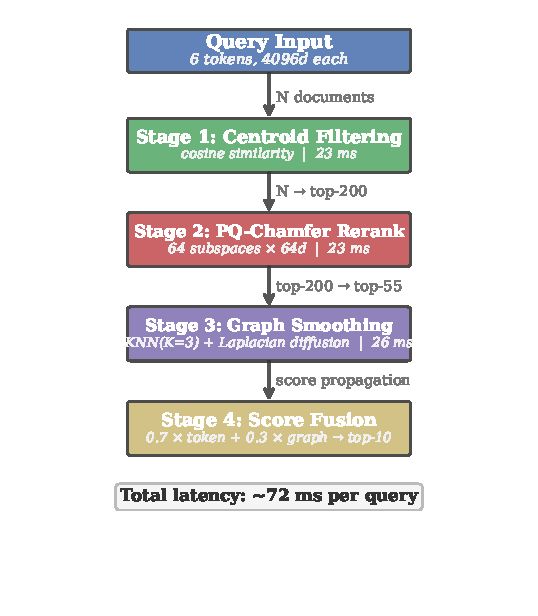
\includegraphics[width=0.5\textwidth]{fig1_pipeline.pdf}
\caption{Overview of the three-stage point cloud retrieval pipeline. Stage~1 performs centroid-based coarse filtering. Stage~2 applies token-level PQ-Chamfer reranking. Stage~3 constructs a KNN graph and applies Laplacian smoothing.}
\label{fig:pipeline}
\end{figure}

\begin{figure}[ht]
\centering
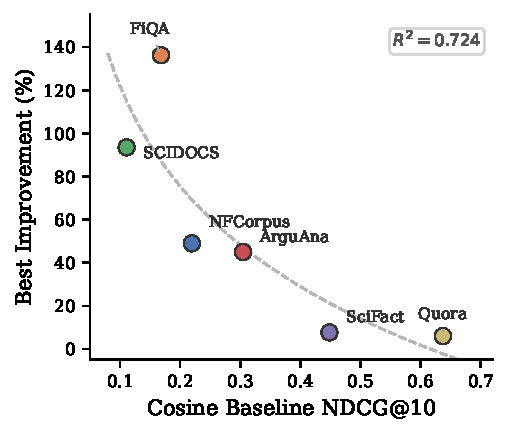
\includegraphics[width=0.5\textwidth]{fig2_scatter.pdf}
\caption{Cosine baseline NDCG@10 (x-axis) versus relative gain from our best pipeline (y-axis) across six BEIR datasets. The strong inverse correlation confirms that our geometric operations recover structural information that becomes redundant as baseline quality improves.}
\label{fig:scatter}
\end{figure}

\begin{figure}[ht]
\centering
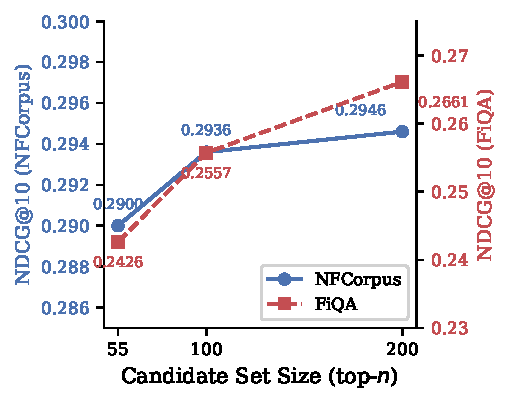
\includegraphics[width=0.5\textwidth]{fig3_topn.pdf}
\caption{Effect of candidate set size (top-$n$) on NDCG@10 for different pipeline configurations on NFCorpus. Token two-stage and fusion achieve stable performance across a wide range of candidate sizes.}
\label{fig:topn}
\end{figure}

% ============================================================
% References
% ============================================================
\bibliographystyle{plainnat}
\bibliography{references}

% ============================================================
\appendix
\section{Complete Falsification Record}
\label{app:falsification}
% ============================================================

The 21 falsified approaches summarized in Table~\ref{tab:falsification} are documented in full---including experimental configurations, quantitative results, and root-cause analyses---in the project repository. Each entry records the hypothesis, experimental setup, observed result, and diagnostic explanation.

Repository: \url{https://github.com/yifanchen/shape-cfd} (to be made public upon publication).

The falsification log follows a structured format: (1)~\textbf{Hypothesis} stated before the experiment; (2)~\textbf{Protocol} specifying parameters, datasets, and metrics; (3)~\textbf{Result} with quantitative measurements; (4)~\textbf{Root-cause analysis} explaining \textit{why} the approach failed, not merely \textit{that} it failed. We believe this level of documentation is valuable for the community: negative results in retrieval are rarely published, yet they constrain the design space and prevent redundant exploration.

\end{document}
